\documentclass[12pt, letterpaper]{article}
\usepackage{graphicx}
\usepackage[ngerman]{babel}
\usepackage{hyperref}
\usepackage{vhistory}
\usepackage{longtable}

\graphicspath{{./img/}}

\title{Technische Dokumentation}
\author{Max Riedel \and Tony Nutzmann \and Matthias Enderlein}

\begin{document}
    \begin{titlepage}
        \clearpage
        \begin{center}
        {\Large Technische Dokumentation}\\[3mm]
        {\Huge Jinba}\\[20mm]

        {vorgelegt von}\\[2mm]
        {\large Max Riedel}\\[2mm]
        {\large Tony Nutzmann}\\[2mm]
        {\large Matthias Enderlein}\\[50mm]

        
\includegraphics[width=75mm]{img/Technische_Hochschule_Brandenburg_Logo.svg.png}\\[10mm]

        {Technische Hochschule Brandenburg}\\[2mm]

        {Fachbereich Informatik}\\[2mm]

        {Studiengang Informatik}\\[20mm]

        {Betreuer \\[2mm] Ilonka Wolpert M.Sc.}
        \end{center}

        \thispagestyle{empty}
    \end{titlepage}

    \begin{versionhistory}
        \vhEntry{0.1}{28.6.2023}{Max Riedel}{Erstellung}
        \vhEntry{0.2}{5.7.2023}{Matthias Enderlein}{Füge ER-Diagramm und 2 Sequenzdiagramme hinzu und korrigiere einige Fehler}
        \vhEntry{1}{6.7.2023}{Tony Nutzmann}{Füge ein Sequenzdiagramm hinzu und korrigiere einige Fehler}
    \end{versionhistory}
    \newpage
    \tableofcontents
    \newpage
    \section{Einführung}

    Das Projekt Jinba, ist eine Jobplattform, die es Jobsuchenden und Unternehmen
    erleichtern soll zusammen zu finden und eine erste Kommunikationsaufnahme zu erreichen.
    Um das zu erreichen, soll die Vermittlung vorrangig über die Fähigkeiten (Skills) der Jobsuchenden
    und geforderten Fähigkeiten in den Jobangeboten eines Unternehmens erfolgen.

    Dabei ist wichtig anzumerken, dass die Plattform keinen kompletten Bewerbungsprozess
    abbilden soll, sondern nur die erste Kontaktaufnahme zwischen Unternehmen und Jobsuchenden.

    \newpage
    \section{Anwendungsfälle}
    

    \subsection{Akteure}

    \begin{table}[htbp]
        \label{tab:aktoren}
        \begin{tabular}{|p{.25\textwidth}|p{.70\textwidth}|}
            \hline
            \textbf{Akteur} & \textbf{Beschreibung} \\
            \hline
            \hline
            Jobsuchender & Ein Jobsuchender ist eine Person, die auf der Suche nach einem Job ist. \\
            \hline
            Unternehmen & Ein Unternehmen ist eine Organisation, die Jobs anbietet. \\
            \hline
        \end{tabular}
        \caption{Liste der Aktoren}
    \end{table}

    \subsection{Anwendungsfälle}

    \begin{longtable}[htbp]{|p{.20\textwidth}|p{.20\textwidth}|p{.40\textwidth}|p{.10\textwidth}|}
       
        \hline
        \textbf{Usecase}&\textbf{Akteur}&\textbf{Beschreibung}&\textbf{Fertig}\\
        \hline
        \hline
        \endfirsthead

        \hline
        \textbf{Usecase}&\textbf{Akteur}&\textbf{Beschreibung}&\textbf{Fertig}\\
        \hline
        \hline
        \endhead

        \hline
        \endfoot

        \hline
        \caption{Anwendungsfälle}  \label{tab:Anwendungsfaelle} 
        \endlastfoot
        Registrierung& Jobsuchender, Unternehmen & Ein Benutzer kann sich auf der Plattform registrieren. & Ja \\
        \hline
        Anmeldung& Jobsuchender, Unternehmen & Ein Benutzer kann sich auf der Plattform anmelden. & Ja \\
        \hline
        Profil bearbeiten& Jobsuchender, Unternehmen & Ein Benutzer kann sein Profil bearbeiten. & Ja \\
        \hline
        Profil anzeigen& Jobsuchender, Unternehmen & Ein Benutzer kann sein Profil anzeigen. & Ja \\
        \hline
        Nach Jobs suchen& Jobsuchender & Ein Jobsuchender kann nach Jobs suchen. & Ja \\
        \hline
        Jobs vorgeschlagen bekommen& Jobsuchender & Ein Jobsuchender kann Jobs vorgeschlagen bekommen. & Ja \\
        \hline
        Jobangebot erstellen& Unternehmen & Ein Unternehmen kann ein Jobangebot erstellen. & Ja \\
        \hline
        Jobangebot bearbeiten& Unternehmen & Ein Unternehmen kann ein Jobangebot bearbeiten. & Ja \\
        \hline
        Jobangebot anzeigen& Jobsuchender, Unternehmen & Ein Benutzer kann ein Jobangebot anzeigen. & Ja \\
        \hline
        Bewerben& Jobsuchender & Ein Jobsuchender kann sich auf ein Jobangebot bewerben. & Ja \\
        \hline
        Bewerbung ansehen& Unternehmen & Ein Unternehmen kann sich die Bewerbungen auf ein Jobangebot ansehen. & Ja \\
        \hline
        Bewerbung annehmen& Unternehmen & Ein Unternehmen kann eine Bewerbung auf ein Jobangebot annehmen. & Ja \\
        \hline
        Bewerbung ablehnen& Unternehmen & Ein Unternehmen kann eine Bewerbung auf ein Jobangebot ablehnen. & Ja \\
    \end{longtable}

    \newpage
    \section{Technische Umsetzung}

    \subsection{Technologien}

    \begin{itemize}
        \item Datenbank: MySQL 8
        \item Programmiersprache: Java 17
        \item Framework: Spring Boot 3.0.6
        \item Template Engine: Thymeleaf
        \item Authentifizierung: Sessions mit Spring Security
        \item Frontend: HTML, CSS, JavaScript
        \item CSS-Framework: CoreUI 4
        \item Build-Tool: Maven
    \end{itemize}

    \newpage
    \subsection{Architektur}

    Die Abbildung \ref{fig:Architektur} veranschaulicht unsere Architektur. Wir haben uns für eine 3 bzw. 5 Schichten Architektur entschieden.
    Die 3 zentralen Schichten bestehen aus:
    \begin{itemize}
        \item Präsentationlayer mit den Controllern
        \item Businesslayer mit den Services
        \item Data Access Layer mit den Repositories
    \end{itemize}

    Drumherum gibt es dann noch zum einen die View Schicht, welche für das Rendern der HTML-Seiten zuständig ist. Und zum anderen
    die Persistenzschicht, welche bei uns eine MySQL Datenbank ist.


    \begin{figure}[htbp]
        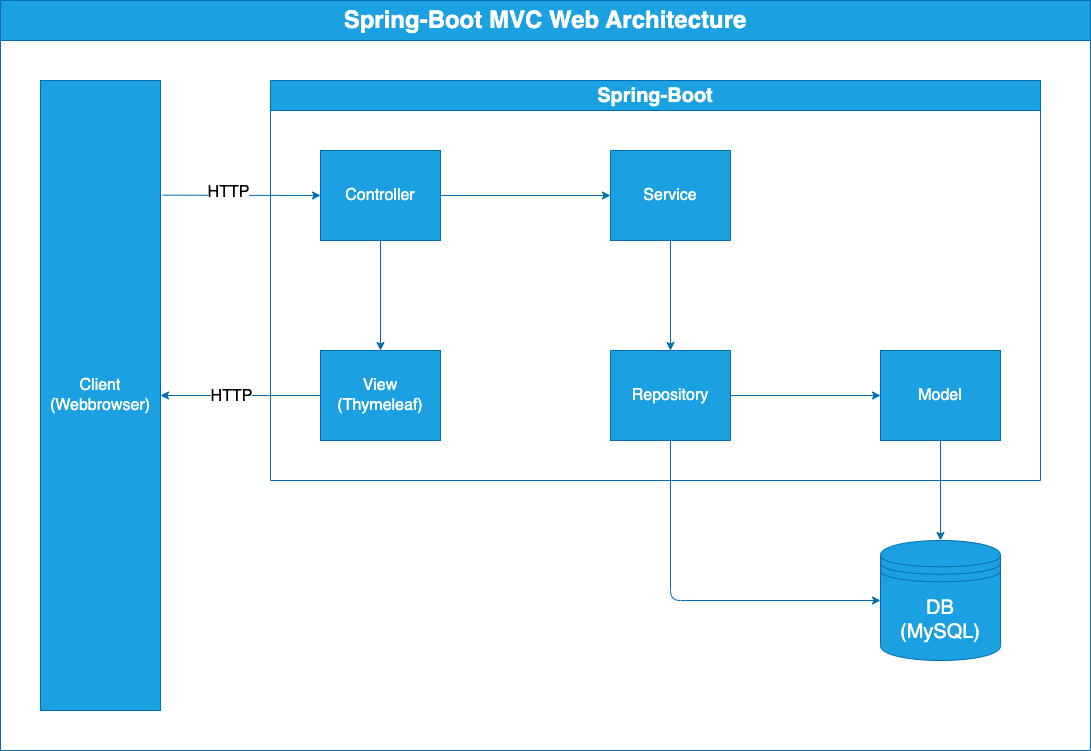
\includegraphics[width = \linewidth]{Architektur.png}
        \caption{Architekturdiagramm}
        \label{fig:Architektur}
    \end{figure}
    
    \subsection{Entity Relationship Diagramm}

    In Abbildung \ref{fig:ERM} ist das ER-Diagramm zu sehen. Es zeigt die Beziehungen zwischen den einzelnen Entitäten.
    Als zentraler Benutzer, existiert ein 'AppUser', der sowohl ein Jobsuchender als auch ein Unternehmen sein kann.
    Das wird durch seine Rolle bestimmt. 
    
    Ein Jobsuchender kann sich auf ein Jobangebot ('JobOffer') bewerben ('JobApplication'). Zudem kann er 
    seine Fähigkeiten ('Skill') angeben. Das wird mittels einer Verknüpfungstabelle ('AppUserSkill') realisiert, die zudem
    das Level des Skills speichert.

    Ein Unternehmen wird von einem AppUser administriert. Dieser kann dann für das Unternehmen ein Jobangebot erstellen ('JobOffer'). Dabei kann es Skills ('Skill') angeben, die ein Jobsuchender
    haben sollte. Auch hier wird das Level des Skills gespeichert ('JobOfferSkill').
    \\[4mm]
    \begin{figure}[htbp]
        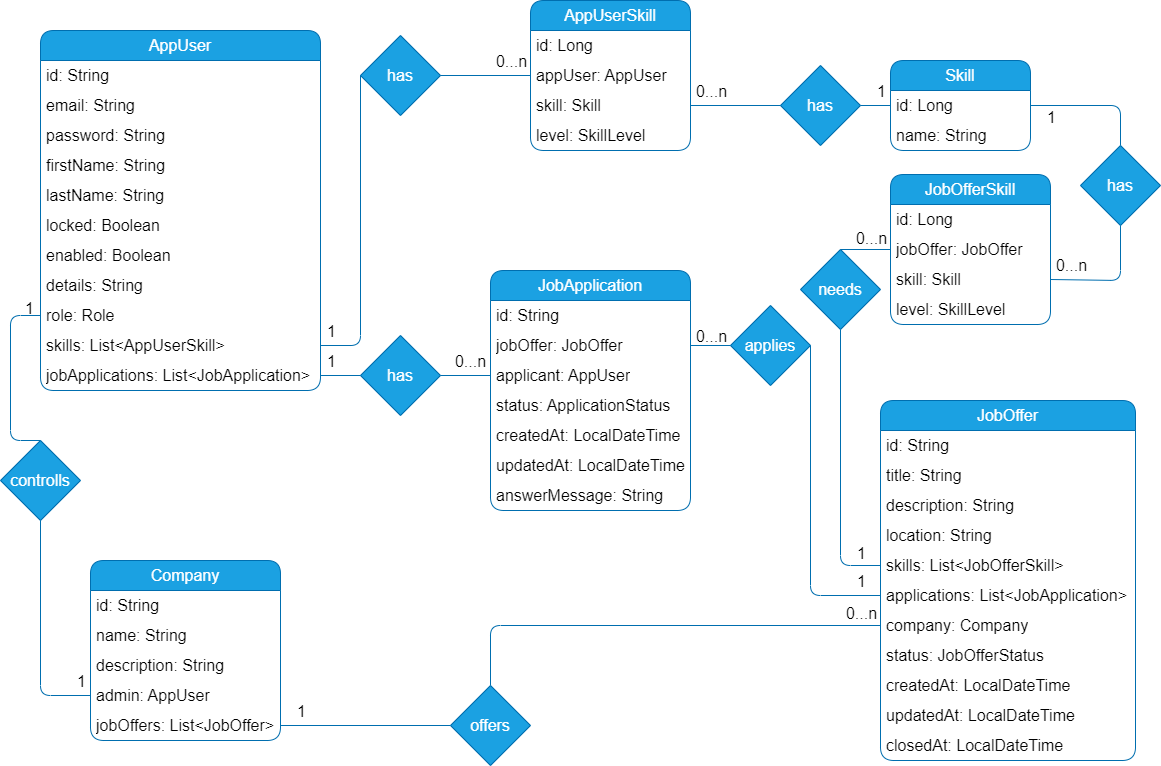
\includegraphics[width = \linewidth]{ERM.png}
        \caption{Entity Relationship Diagramm}
        \label{fig:ERM}
    \end{figure}
    

    \subsection{Sequenzdiagramme}
    
    Im Folgenden sind Sequenzdiagramme für drei wichtige Anwendungsfälle zu sehen. In diesen wird die Kommunikation zwischen
    den verschieden Schichten der Anwendung dargestellt. Die Abbildungen \ref{fig:Apply} bis \ref{fig:Accept} liegen im Anhang bei.

    \subsubsection{Bewerben}

    Die Abbildung \ref{fig:Apply} zeigt den Kommunikationsablauf, wenn sich ein Jobsuchender auf ein Jobangebot bewirbt. Dafür muss zuerst
    der aktuell angemeldete Benutzer ermittelt werden, dann wird eine neue Bewerbung erstellt und in der Datenbank gespeichert.

    \begin{figure}[h!]
        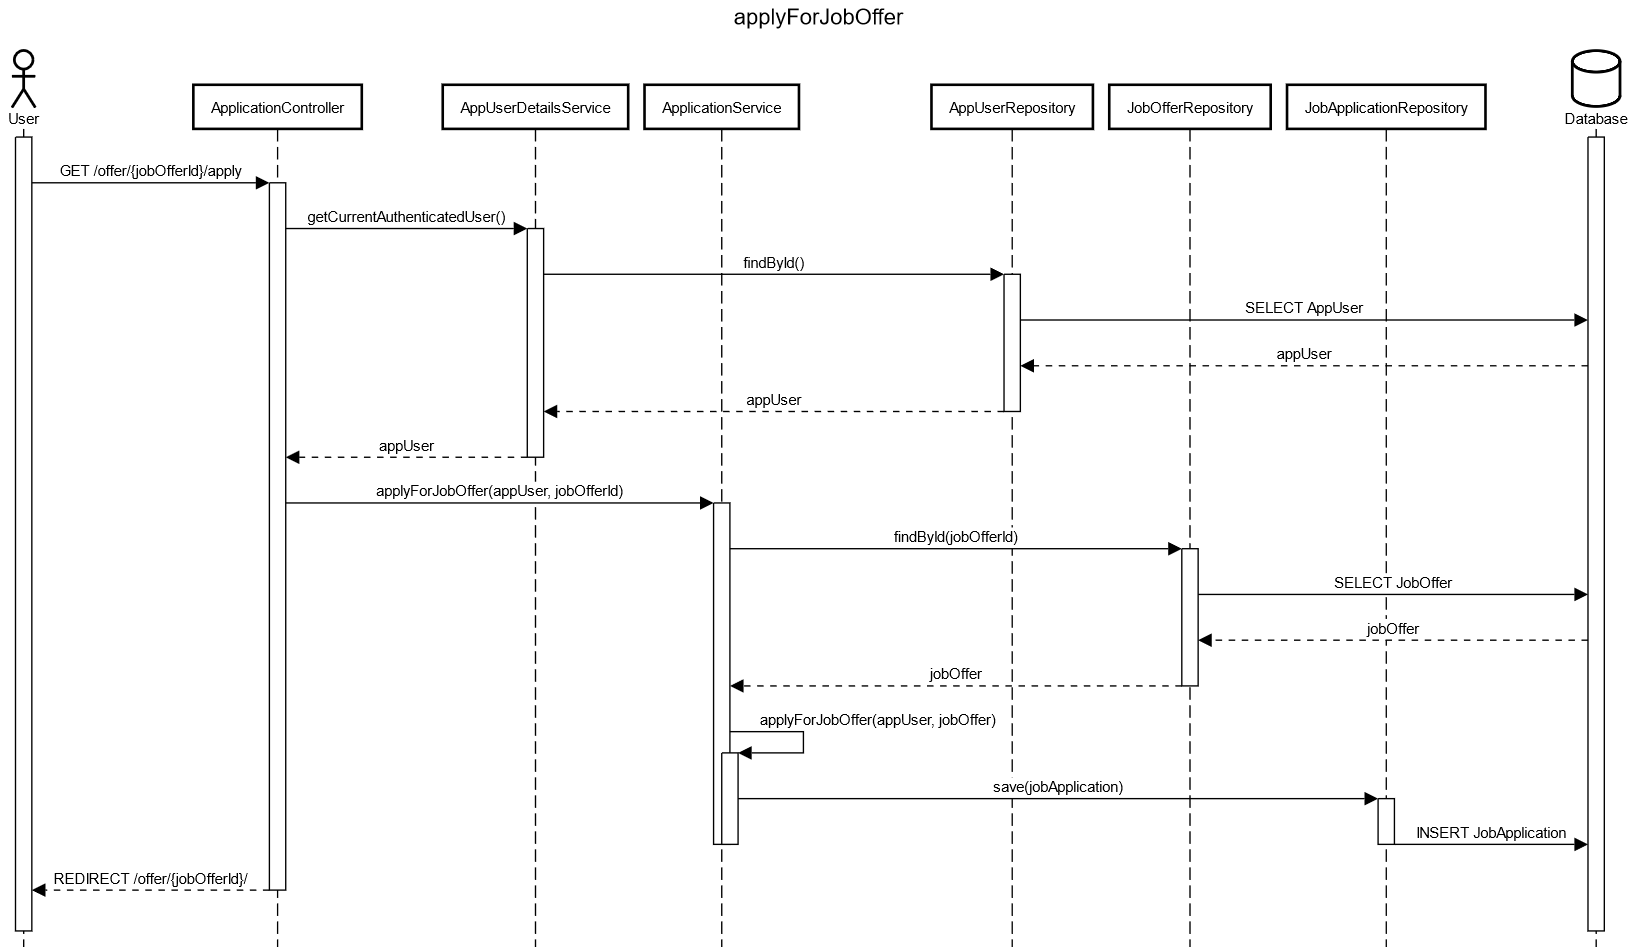
\includegraphics[width = \linewidth]{sequence/applyForJobOfferSequenzDiagramm.png}
        \caption{Sequenzdiagramm - Bewerben}
        \label{fig:Apply}
    \end{figure}

    \subsubsection{Jobangebot erstellen}

    Die Abbildung \ref{fig:CreateJobOffer} zeigt den Kommunikationsablauf, wenn ein Unternehmen ein Jobangebot erstellt. Dafür muss zuerst
    die Firma des aktuell angemeldeten Benutzers ermittelt werden. Anschließend wird ein neues Jobangebot erstellt, mit den im Formular
    übermittelten Daten. Dabei ist zu beachten, dass die Skills, die noch nicht existieren, erstmal erstellt werden müssen
    und dann dem Jobangebot hinzugefügt werden. Zuletzt wird das Jobangebot in der Datenbank gespeichert.

    \begin{figure}[h!]
        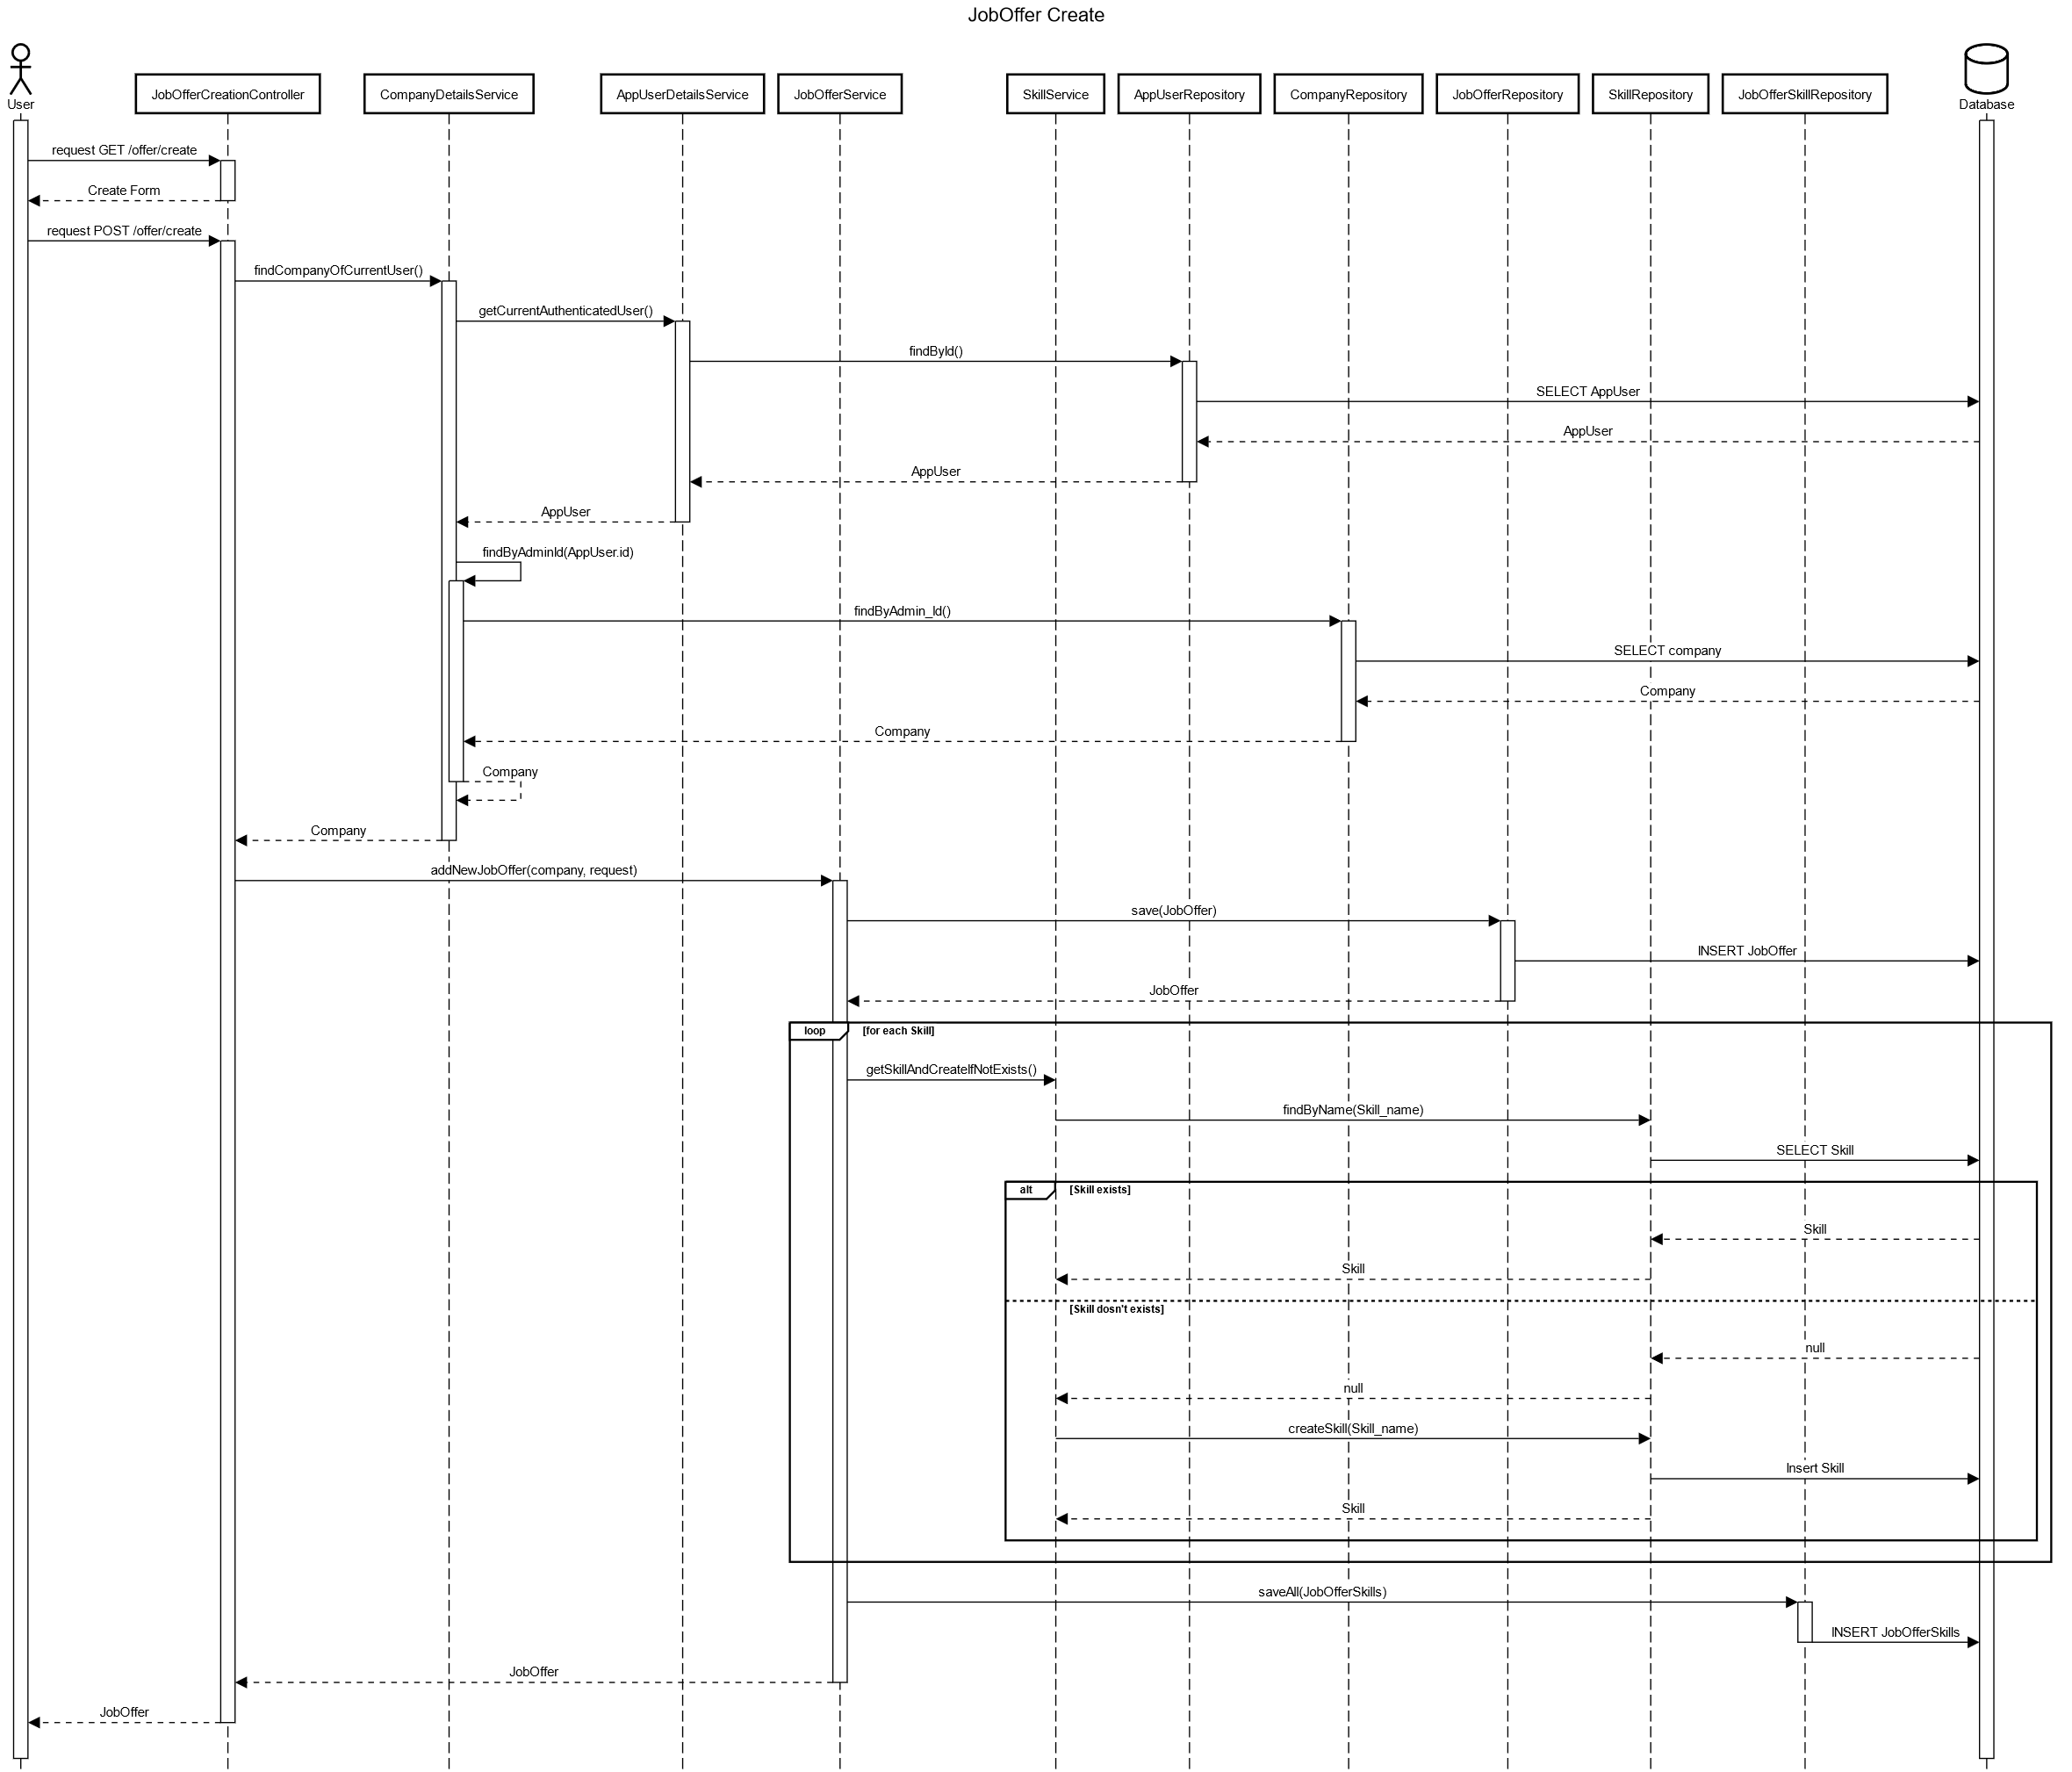
\includegraphics[width = \linewidth]{sequence/JobOfferCreateSequenzDiagramm.png}
        \caption{Sequenzdiagramm - Jobangebot erstellen}
        \label{fig:CreateJobOffer}
    \end{figure}




    \subsubsection{Bewerbung annehmen}

    Die Abbildung \ref{fig:Accept} zeigt den Kommunikationsablauf, wenn ein Unternehmen eine Bewerbung auf ein Jobangebot annimmt. Dafür muss zuerst
    der aktuell angemeldete Benutzer ermittelt werden, um zu überprüfen, dass auch nur der Admin die Bewerbung annimmt. 
    Dann wird die Bewerbung aus der Datenbank geladen, der Status auf 'ACCEPTED' gesetzt und die vom Admin übermittelte Nachricht eingetragen.
    Zuletzt wird die Bewerbung wieder in der Datenbank gespeichert.
    \begin{figure}[h!]
        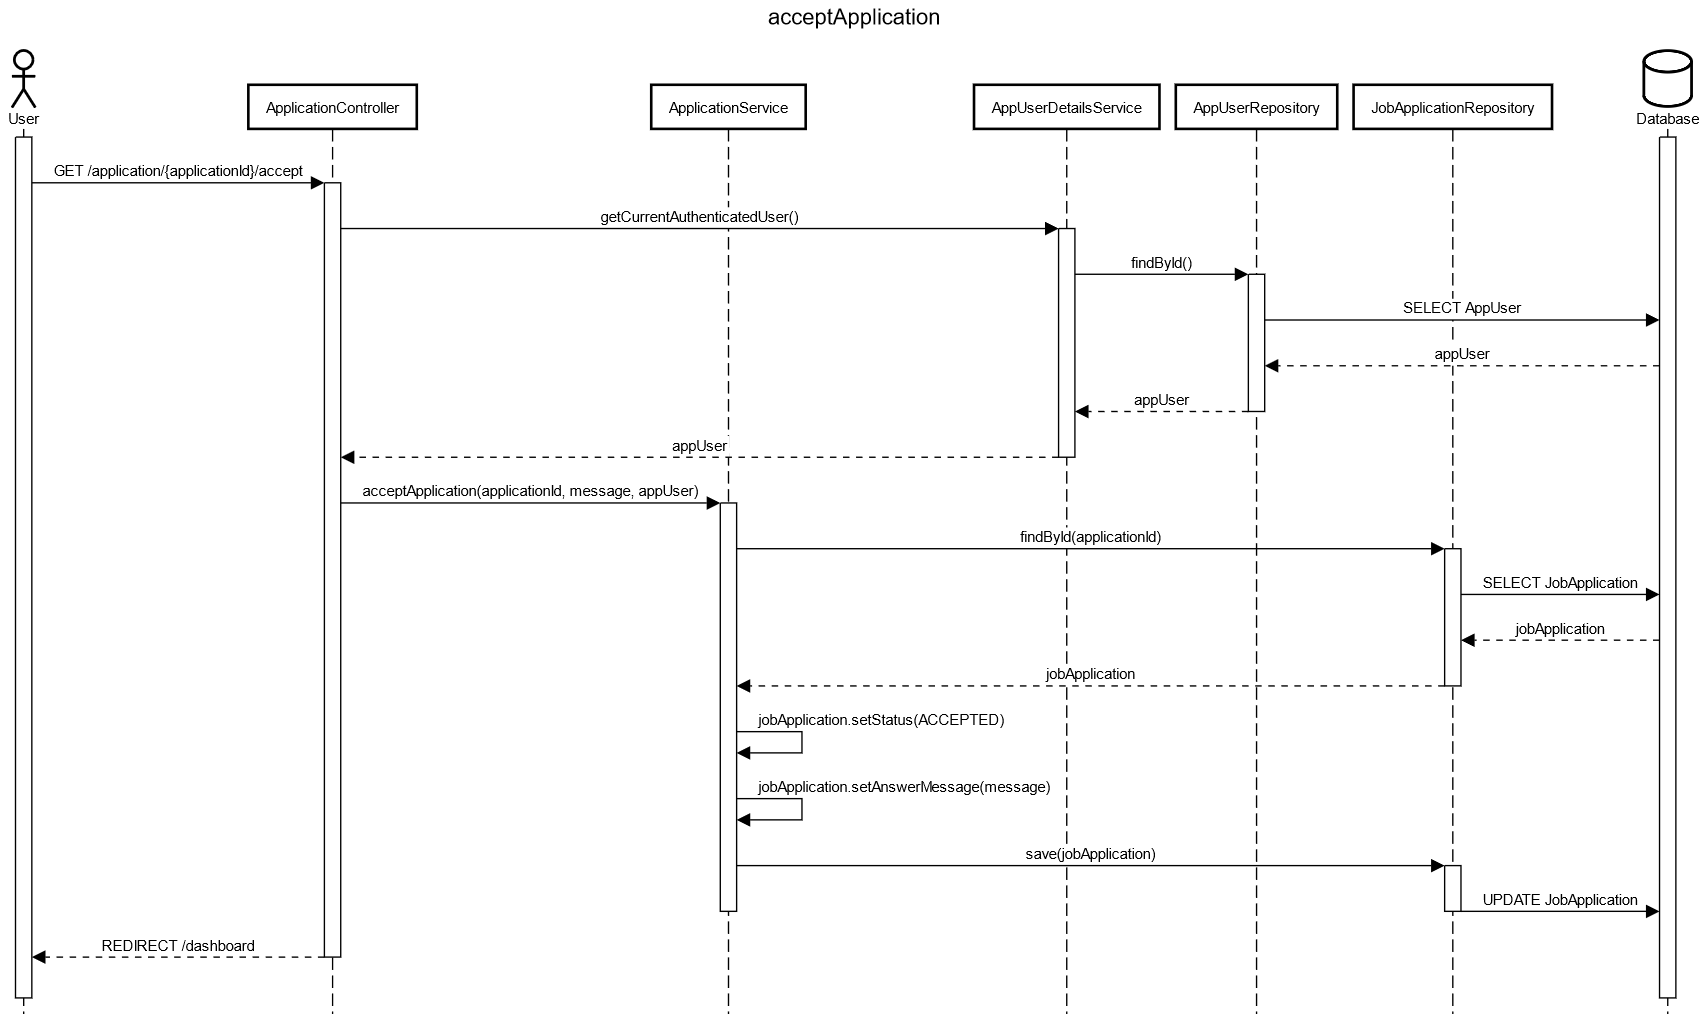
\includegraphics[width = \linewidth]{sequence/acceptApplicationSequenzDiagramm.png}
        \caption{Sequenzdiagramm - Bewerbung annehmen}
        \label{fig:Accept}
    \end{figure}
\end{document}